\section{Ordered array of particles}

Following the strategy of \citet{loisy} This appendix treat the case of ordered array of particles. 

Eventhrougth not realistic, the advantage is that in these simulations we do not have any particle-particle interaction.
It is therefore of a great interest to evaluate different properties knowing that 
\begin{figure}[h!]
    \centering    
    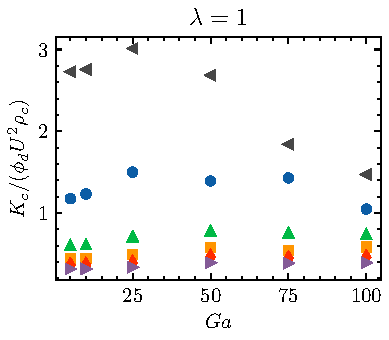
\includegraphics[height = 0.35\textwidth]{image/HOMOGENEOUS/fCA/Tf_N_1_l_1.pdf}
    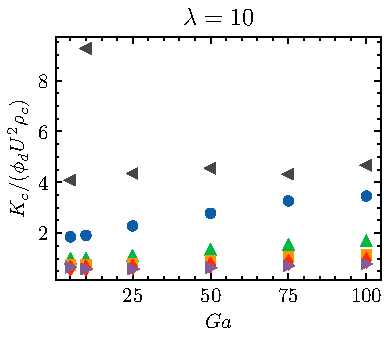
\includegraphics[height = 0.35\textwidth]{image/HOMOGENEOUS/fCA/Tf_N_1_l_10.pdf}

    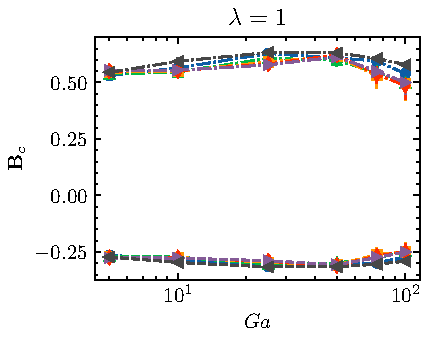
\includegraphics[height = 0.35\textwidth]{image/HOMOGENEOUS/fCA/Bf_N_1_l_1.pdf}
    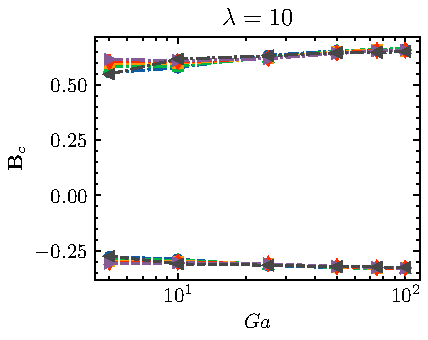
\includegraphics[height = 0.35\textwidth]{image/HOMOGENEOUS/fCA/Bf_N_1_l_10.pdf}

    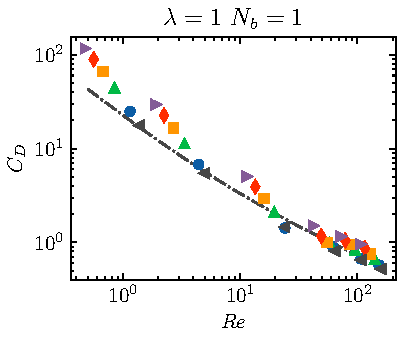
\includegraphics[height = 0.35\textwidth]{image/HOMOGENEOUS/fCA/Cp_N_1_l_1.pdf}
    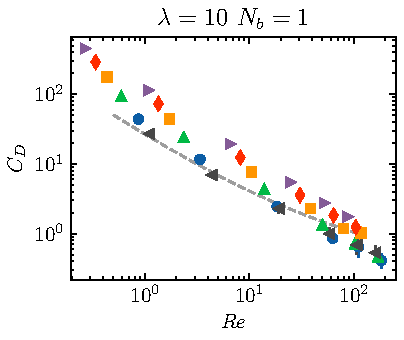
\includegraphics[height = 0.35\textwidth]{image/HOMOGENEOUS/fCA/Cp_N_1_l_10.pdf}
    \caption{
        (top) dimensionless fluid pseudo turbulent energy. 
        (middle) deviatoric components of the matic B
        (bottom) 
        Drag coefficient and dimensionless force for ordered array. 
        (--) Empirical formula of Rvikind and Ryskin (1976)
        The symbols correspond to different volume fraction ($\blacktriangleleft$) $\phi = 0.1$\%, ($\bullet$) $\phi = 1\%$, ($\blacktriangle$) $\phi = 5\%$, ($\blacksquare$) $\phi = 10\%$, ($\blacklozenge$) $\phi = 15\%$, and ($\blacktriangleright$) $\phi = 20$\%.
    }
    \label{fig:Cp}
\end{figure}


On \ref{fig:Cp}(bottom) we can see that the formula of Rvikind and Ryskin (1976) is valid only in the low inertial regime which is probably due to the wake of the particles in tri periodic domain. Pseudo_turb/Ordered.tex